\documentclass{article}

\usepackage[table]{xcolor}
\usepackage{amsmath, physics, gensymb, microtype, float, multicol, fancyhdr, hyperref}
\usepackage{tikz, tikz-3dplot, pgfplots}
\usepackage[letterpaper, bottom=1in, top=1in, left=1in, right=1in]{geometry}

\pgfplotsset{compat=newest}

\newcommand{\dt}{\mathrm{d}t}
\newcommand{\x}{\mathrm{x}}
\newcommand{\y}{\mathrm{y}}
\newcommand{\z}{\mathrm{z}}
\newcommand{\vel}{\mathrm{v}}
\newcommand{\ddt}[1]{\frac{\mathrm{d}#1}{\dt}}
\newcommand{\dydt}{\frac{\mathrm{d}y}{\dt}}

\patchcmd\subequations
 {\theparentequation\alph{equation}}
 {\subequationsformat}
 {}{}
\newcommand{\subequationsformat}{\theparentequation.\arabic{equation}}

\pagestyle{fancy}

\title{Report 1: Measurements}
\date{2/10/2023}
\author{Laith Toom}

\begin{document}
\maketitle 

\noindent Phys 207 Lab CD4

\noindent \textbf{Instructor:} Georgios Goulas

\noindent \textbf{Group:} Radjabov Jake and Tenzin Tsepak

\vspace{1em}
\hrule
\section{Introduction}
This lab is meant to explore the relationship between different variables, 
or the lack thereof.

\vspace{1em}
\hrule
\section{Procedure}

\subsection{Head Circumference and Heartbeat Time}
Each group will pick one of their members to be their test subject. First, we will measure the 
circumference of their head by using a rope and a ruler in cm. Then, we will time between 
two of their heartbeats. We will enter this data onto the computer to use at the end of the lab.

\subsection{Estimate $\pi$}
We are meant to find the circumference and diamater of various objects, then calculate 
the ratio between the two using the formula:
\[ \frac{C}{D}=\pi \]
The calculated value will only be an esimate of $\pi$, but it should be relatively close.

\subsubsection{3 Objects}
There are 3 circular objects:
\begin{enumerate}
    \item A 500-gram mass.
    \item A small circular disk.
    \item A large circular disk.
\end{enumerate}
For each object, we measure their circumference and diameter using a ruler, in which these values
will be recorded in a Microsoft Excel spreadsheet. Then, we create a scatter plot in Excel, with 
the $x$-axis representing diameter and the $y$-axis representing circumfernece. Our estimate 
of $\pi$ for this test will be the slope of the trendline of our poltted data.

\subsubsection{Toothpicks}
We form a circular shape using toothpicks. The circumference will be the amount 
of toothpicks used to form the shape and the diameter will be roughly the amount 
of toothpicks it takes to divide the shape in half. We then calculate our $\pi$ 
estimate using these measurements.

\subsubsection{Google Maps}
We will find a circular building or geographic location. Then, using the measure
distance feature of Google Maps, plot points around the circumference of the object to 
find the circumference and plot two points perpendicular to each other as well as the center of 
the object to find the diameter. We will then calculate our estimate of $\pi$ using these 
measurements.

\subsection{Calculate Uncertainty in Measurements}
We will calculate the potential uncertaintiy in measuring length using the formula:
\begin{align}
    A \pm \delta A = (A)\left[1\pm\frac{\delta A}{A}\right]
\end{align}
and density using the formula:
\begin{align}
    \left(\frac{A\pm\delta A}{B\pm\delta B}\right) = \left(\frac{A}{B}\right)\left[1\pm\left(\frac{\delta A}{A}+\frac{\delta B}{B}\right)\right]\label{eq:2}
\end{align}

\subsubsection{Measure the Fish}
We will measure the length of a printed image of a fish using a ruler in centimeters. Then, we will calculate
the uncertaintiy of this measurement by taking the ± difference of the ticks on the ruler nearest to our
measurement and dividing the difference in half.

For example, if our measurement was 10.2 cm, and assuming our ruler measured in intervals of 0.5 cm, we
would subtract the tick to the left (10.0 cm) from the tick to the right (10.5 cm), and divide that difference
(0.5 cm) by 2 to get 0.25 cm. Then, since our measurement could be greater or less than the actual length,
we would write our value as ±0.25 cm.

\subsubsection{Density of Wood Block}
We will calculate the density of a mysterious wood block using the formula:
\[ p = \frac{m}{v}\]
Where $p$ is density, $m$ is mass, and $v$ is volume. 
We will calculate the mass in grams of the wood block using a digital scale. 
In order to calculate volume, we will measure the length, width, and height of 
the wood block in centimeters using a ruler, then multiply all three dimensions to 
get our volume in $\mathrm{cm}^3$.

\subsection{Time of Oscillations}
We will measure the time it takes for a pendulum to swing back and forth, which is known 
as the \emph{period of oscillation}. The pendulum will be 1.5 m long, in which it will be a rope tied 
to a 500-gram weight, with the length of the pendulum being the length of the rope plus the 
distance from the end of the rope to the center of mass of our 500-gram weight.

We will record the time it takes for this pendulum to oscillate, then reduce the length of 
the pendulum. We will repeat this 4 more times until we have 5 measurements. Both the length 
and period of oscillation in a Excel spreadsheet, then plot the values in which the period of 
oscillation will be a function of length.  

\subsection{Experiment Analysis}
Going back to the first part of the procedure, we will create a table in Excel using 
those measurements, and then create a scatter plot the measurements. The $x$-axis will 
be heartbeat time and the $y$-axis will be head circumference. 

\vspace{1em}
\hrule
\section{Data and Calculations}

\subsection{Figures and Tables}
\subsubsection{Pi Estimates}
\begin{figure}[H]
    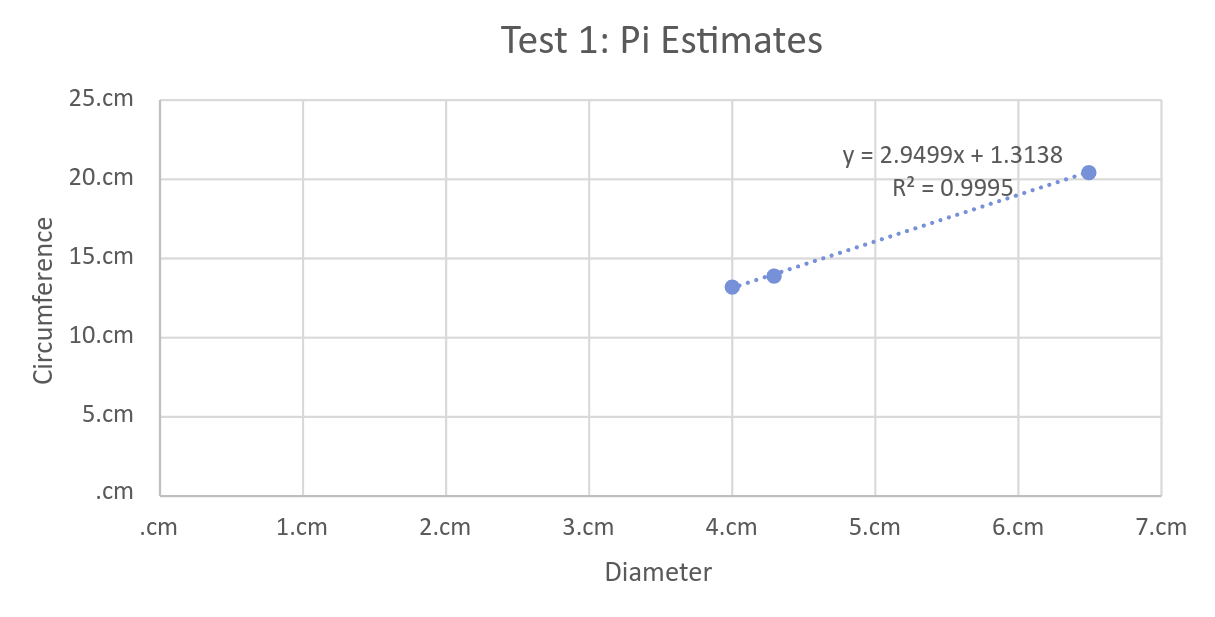
\includegraphics[width=16cm]{lab1_plot1.png}
    \caption{Circumference vs. Diamater of 3 Objects}
    \label{plot:1}
\end{figure}

\setlength{\tabcolsep}{18pt}
\renewcommand{\arraystretch}{1.5}
\begin{table}[H]
\centering
\begin{tabular}{|c|c|c|}
    \hline
    \rowcolor{black}
    \color{white} Object \# & \color{white} Diamater (cm) & \color{white} Circumference (cm) \\
    \hline
    1 & 4.0 cm & 13.2 cm \\
    \hline
    2 & 6.5 cm & 20.5 cm \\
    \hline
    3 & 4.3 cm & 13.9 cm \\
    
    \hline
\end{tabular} 
\caption{Diamater and Circumference of 3 Objects}
\end{table}

\subsubsection{Oscillation and Pendulum Length}
\begin{figure}[H]
    \includegraphics*[width=16cm]{lab1_plot3.png}
    \caption{Period of Oscillation vs. Pendulum Length}
    \label{plot:2}
\end{figure}

\begin{table}[H]
\centering
\begin{tabular}{|c|c|}
    \hline
    \rowcolor{black}
    \color{white} Rope Length (cm) & \color{white} Period of Oscillation (s) \\
    \hline
    149.1 cm & 2.46 s \\
    \hline
    129.1 cm & 2.28 s \\
    \hline
    109.1 cm & 1.99 s \\
    \hline
    89.1 cm  & 1.79 s \\
    \hline
    79.1 cm  & 1.61 s \\

    \hline
\end{tabular} 
\caption{Rope Length vs. Period of Oscillation}
\end{table}

\subsubsection{Density of Wood}
\begin{table}[H]
\centering
\begin{tabular}{|c|c|c|}
    \hline
    \rowcolor{black}
    \color{white} Mass (g) & \color{white} Volume ($\mathrm{cm}^3$) & \color{white} Density ($\mathrm{g}/\mathrm{cm}^3$) \\
    \hline
    72.3 g & 122.14 $\mathrm{cm}^3$ & 0.59 $\mathrm{g}/\mathrm{cm}^3$ \\

    \hline
\end{tabular} 
\caption{Mass, Volume, and Density of Wood Block}
\end{table}

\subsubsection{Time Between Heartbeats vs Head Circumference}
\begin{figure}[H]
    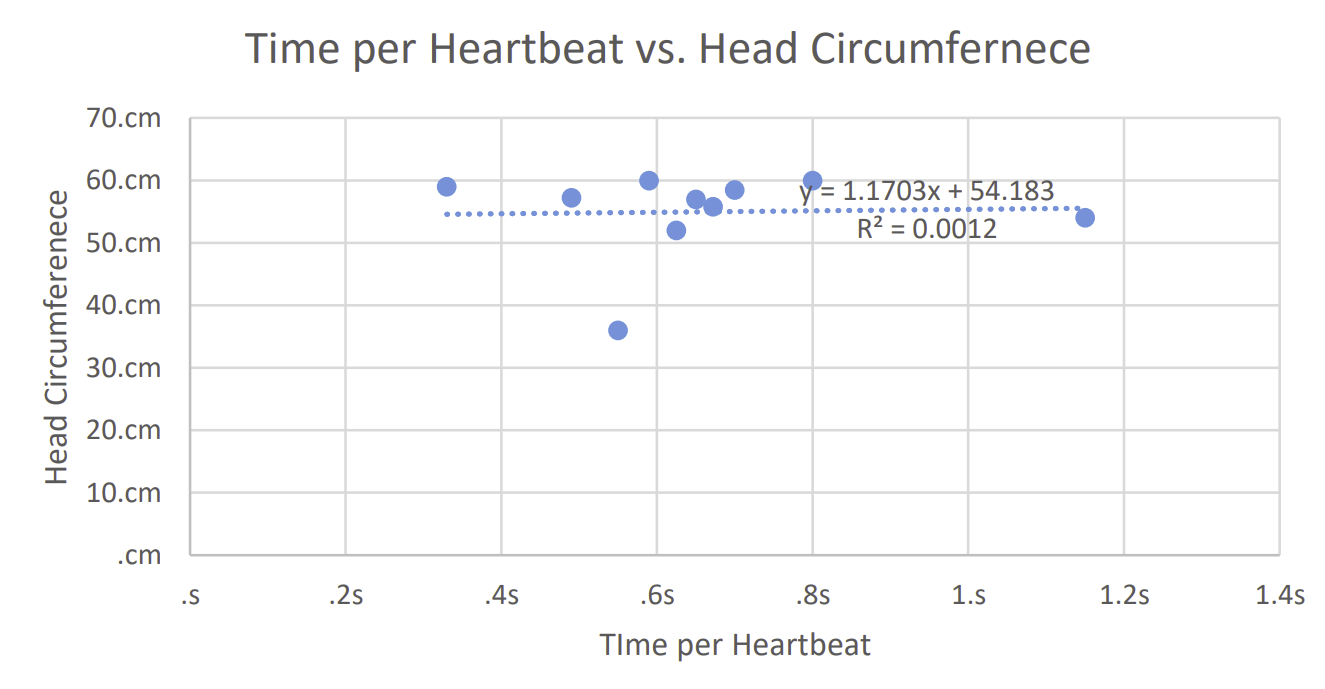
\includegraphics[width=16cm]{lab1_plot2.png}
    \caption{Heart Pulse vs. Head Circumference}
    \label{plot:3}
\end{figure}

\begin{table}[H]
\centering
\begin{tabular}{|c|c|}
    \hline
    \rowcolor{black}
    \color{white} Time Between Heartbeats (s) & \color{white} Head Circumference (cm) \\
    \hline
    0.8 s  & 60.0 cm \\
    \hline
    0.59 s & 60.0 cm \\
    \hline
    0.33 s & 59.0 cm \\
    \hline
    0.7 s  & 58.5 cm \\
    \hline
    0.49 s & 57.2 cm \\
    \hline
    0.65 s & 57.0 cm \\
    \hline
    0.67 s & 55.8 cm \\
    \hline
    1.15 s & 54.0 cm \\
    \hline
    0.63 s & 52.0 cm \\
    \hline
    0.55 s & 36.0 cm \\

    \hline
\end{tabular} 
\caption{Time Between Heartbeats vs. Head Circumference}
\end{table}

\subsection{Calculations}
\subsubsection{Density of Wood Block}
The dimensions of the wood block were:
\[ l = 23.8\,\mathrm{cm} \quad w = 5.448\,\mathrm{cm} \quad  h = 0.942\,\mathrm{cm}\]
Thus the volume was:
\[ 
    v = 
    l\cdot w \cdot h = 
    23.8\,\mathrm{cm} \cdot 5.448\,\mathrm{cm} \cdot 0.942\,\mathrm{cm} 
    \approx122.14\,\mathrm{cm}^3
\]
The mass of the wood block was $m=72.3$ g, thus the density was:
\[
    p = \frac{m}{v} = \frac{72.3\,\mathrm{g}}{122.14\,\mathrm{cm}^3} \approx 0.59 \,\mathrm{g/cm}^3    
\]
\subsubsection{Uncertainty in Density of Wood Block}
Since the density $p$ consists of two quantities: mass $m$, which was measured using a scale 
measuring in increments of 0.01 grams, and volume $v$, which was calculated using the product of 
the 3 measured dimensions $l,\,w,\,$ and $h$, all measured using a caliper measuring in increments 
of 0.001 centimeters. 

The error propagation of the mass, which will be the $\delta A$ of formula \eqref{eq:2}, 
can be calculated by dividing the increment of measurement by 2:
\[ \delta A = \pm\frac{0.01\,\mathrm{g}}{2} = \pm0.05\,\mathrm{g} \]
The error propagation of the volume $\delta B$ will require us to calculate the relative uncertainties
of all 3 measured dimensions. 

\noindent The relative uncertainty of length $l$:
\[ \delta l = \pm\frac{0.001 \,\mathrm{cm}}{l} \cdot 100 = \pm\frac{0.001 \,\mathrm{cm}}{23.8 \,\mathrm{cm}} \cdot 100 \approx \pm0.0042017\,\% \]
The relative uncertainty of length $w$:
\[ \delta w = \pm\frac{0.001 \,\mathrm{cm}}{w} \cdot 100 = \pm\frac{0.001 \,\mathrm{cm}}{5.448 \,\mathrm{cm}} \cdot 100 \approx \pm0.0183554\,\% \]
The relative uncertainty of length $h$:
\[ \delta h = \pm\frac{0.001 \,\mathrm{cm}}{h} \cdot 100 = \pm\frac{0.001 \,\mathrm{cm}}{0.942 \,\mathrm{cm}} \cdot 100 \approx \pm0.1061571\,\% \]
When we multiply all 3 dimensions, we will add the uncertainties:
\[ v = (l\pm\delta l)(w\pm\delta w)(h\pm\delta h) = lwh\pm(\delta l + \delta w + \delta h) \]
When we substitue in our measurements, we get:
\[ v = 122.14 \,\mathrm{cm}^3 \pm 0.1287142\,\% \]
and converting to absolute uncertainty:
\[ v = 122.14 \pm 15.72 \,\mathrm{cm}^3 \]
Using formula \eqref{eq:2}, we find that our uncertainty is:
\[ p = \frac{72.3\pm0.05\,\mathrm{g}}{122.14\pm15.72\,\mathrm{cm}^3}\]

\vspace{1em}
\hrule

\section{Questions}
\subsection{Discuss the limitations of these 
methods for calculating $\pi$. Which method was 
the best? The worst? Are there improvements to be made?}

The best method for estimating $\pi$ was taking the slope of 
the linear trendline from the plotted diameters and circumferences 
of the three objects. This is so because the value obtained from the
slope had the least difference from $\pi$ compared to the other methods.

Using Google Maps to calculate $\pi$ turned out to be the worst method 
since the calculated value had the biggest difference from $\pi$ compared 
to the other methods.

We could improve the first method of calculation by measuring more than just 
3 objects. Perhaps 6 or 9 would give us a more accurate value. The second method
of calculation, in which we used tooth picks to form a circular shape, would benefit 
from the use of more toothpicks in forming the circumference. It might also benefit 
from forming multiple circular shapes from different amounts of toothpicks, then taking 
the average of the calculated $\pi$ estimates. The third and final method could benefit 
from plotting more points along the circumference of the circular object. 

\subsection{Try to match your piece of wood with a known 
tree. Discuss whether you can be certain of your 
identification.}

\subsection{Based only on your experimental data, can you 
say how the time for one swing relates to the length 
of the pendulum? Is there a clear functional 
dependance? What could you do to make the experiment better?}
Based on my experimental data, the time for one swing seems to have a 
linear relationship to the length of the pendulum. Thus, it is clear that
the period of oscillation depends on the length of the pendulum. The experiment 
would benefit from recording more than 5 data points as well as specifying a specific 
interval of rope length between data points.

\subsection{Is there a correlation between the circumference
of someone's head and the time between heartbeats? Would you 
expect there to be one?}

\vspace{1em}
\hrule
\vspace{1em}
\section{Conclusion}


\end{document}